\chapter{ELEMENTARY PRINCIPLES}
\section{Mechanics of a Particle}
\subsubsection{Linear Momentum}
\begin{align*}
\text{Let $\textbf{r}$ be the radius vector of }&\text{a particle from some given origin and $\textbf{v}$ its vector velocity.}\\
\textbf{v}&=\frac{d\textbf{r}}{dt}\\
\text{The linear momentum }&\text{$\textbf{p}$ of the particle is }\\
\textbf{p}&=m\textbf{v}
\intertext{Newton's second law of motion  states that there exist frames of reference in which the motion of the particle is described by the differential equation}
\textbf{F}&=\frac{d\textbf{p}}{dt}\equiv\dot{\textbf{p}}\\
\textbf{F}&=\frac{d}{dt}(m\textbf{v})\\
\text{If the mass of particle}&\text{ is constant}\\
\textbf{F}&=m\frac{d\textbf{v}}{dt}=m\textbf{a}
\end{align*}
Where $\textbf{a}$ is the vector acceleration of the particle
The equation of motion is thus a differential equation of second order, assuming $\textbf{F}$ does not depend on higher-order derivatives.
\textbf{\textit{Conservation theorem for the Linear Momentum of a Particle: If the total force $\vec{F}$ is zero, then $\dot{\vec{p}}$, is conserved.}}
\subsubsection{Angular Momentum}
\begin{align*}
\text{The angular momentum }&\text{of the particle about point $O$, denoted by $\textbf{L}$, is defined as}\\
\textbf{L}&=\textbf{r}\times\textbf{p}\\
\text{where $\textbf{r}$ is the radius vector}&\text{ from $O$ to the particle. The moment of force or torque about $O$}\\
\textbf{N}&=\textbf{r}\times\textbf{F}\\
\textbf{r}\times\textbf{F}&=\textbf{N}=\textbf{r}\times\frac{d}{dt}(mv)\\
\text{ using the vector }&\text{identity}\\
\frac{d}{dt}(\textbf{r}\times m\textbf{v})\textbf{v}\times m\textbf{v}&=\textbf{r}\times\frac{d}{dt}(m\textbf{v})\\
\textbf{N}&=\frac{d}{dt}(\textbf{r}\times m\textbf{v})=\frac{d\textbf{L}}{dt}\equiv \dot{\textbf{L}}\\
\text{Note that both $\textbf{N}$ and }&\text{ $\textbf{L}$ depend on the point $O$ about which the moments are taken.}\\
\end{align*}
\textit{Conservation Theorem for the Angular Momentum of a Particle: If the total torque, $\textbf{N}$,is zero then $\dot{\textbf{L}}=0$, and the angular momentum $\textbf{L}$ is conserved. }
\subsubsection{Energy}
Next consider the work done by the external force $\textbf{F}$ upon the particle in going from point 1 to point 2. \\
This work is 
\begin{align*}
W_{12}&=\int\limits_{1}^{2}\textbf{F}\cdot d\textbf{s}\\
\int\textbf{F}\cdot d\textbf{s}&=m\int\frac{d\textbf{v}}{dt}\cdot\textbf{v}dt=\frac{m}{2}\int\frac{d}{dt}(v^2)dt\\
W_{12}&=\frac{m}{2}(v_2^2-v_1^2)
\end{align*}
The scalar quantity $mv^2/2$ is called the kinetic energy of the particle and is denoted by $T$. so that the work done is equal to the change in the kinetic energy.
\begin{equation}
W_{12} =T_2-T_1\label{EP-01}
\end{equation}
if the force field is such that the work $W_{12}$ is the same for any physically possible path between points 1 and 2, then the force (and the system) is said to be conservative.
\begin{align*}
\text{ or }\quad
\oint\textbf{F}\cdot\textbf{s}&=0\\
\text{$\textbf{F}$ be the gradient }&\text{of some scalar function of position}\\
\textbf{F}&=-\nabla V(\textbf{r})\\
\text{where $V$ is called}&\text{ the potential energy.}\\
\textbf{F}\cdot d\textbf{s}&=-dV\\
\text{or}\quad
F_s&=-\frac{\partial V}{\partial s}
\end{align*}
We can add to $V$ any quantity constant in space, without affecting  the results. Hence the zero level of $V$ is arbitrary.\\
For a consetvative system, the work done by the forces is 
\begin{equation}
W_{12}=V_1-V_2\label{EP-02}
\end{equation}
Combining Eq.(\ref{EP-01}) with Eq.(\ref{EP-02}),we have the result 
$$T_1+V_1=T_2+V_2$$
\textbf{\textit{Energy Conservation Theorem for a Particle: If the forces acting on a particle are consetvative, then the total energy of the particle, $T+V$,is conserved.}}\\
\begin{note}
	The force applied to to a particle may in some circumstances be given by the gradient of a scalar function that depends explicity on both the position of the particle and the time. However, the work done on the particle when it travels a distance $ds$.
	$$\textbf{F}\cdot{d\textbf{s}=\frac{\partial V}{\partial s}ds}$$
	is then no longer the total change in $-V$ during the displacement, since $V$ also changes explicitly with time as the particle moves. Hence, the work done as the particle goes from point 1 to point 2 is no longer the difference in the function $V$ between those points. While a total  energy $T+V$ may still be defined, it is not conserved during the course of the particle's motion.
\end{note}
\section{Mechanics of a System of Particle}
When considering a system of particles, we must distinguish between the external forces acting on the particles due to source outside the system and internal forces on some particle $i$ due to all other particles in the system.
\subsubsection{Linear Momentum}
\begin{align*}
\text{Equation of motion}&\text{ for the $i^{th}$ particle}\\
\vec{F}_i^{(e)}+\sum\limits_{j}\vec{F}_{ji}=\vec{\dot{p_i}}\\
\vec{F}_i^{(e)}\text{- external force}\\
\vec{F}_{ji}-\text{ internal force on  }&\text{the $i^{th}$ particle due to the $j^{th}$ particle.}\\
\text{Assume $\vec{F}_{ij}$ , like ${F}_i^{(e)}$}&\text{ obey Newton's third law  ie. $\vec{F}_{ij}= - \vec{F}_{ji}$,}\\
\text{this assumption some }&\text{times referred to as } \textit{The weak law of action and reaction}\\
\therefore \quad\text{ we get }\quad \frac{d^2}{dt^2}\sum\limits_{i}m_ir_i&=\sum\limits_{i}{F}_i^{(e)}+\sum\limits_{i,j ,\ i\neq j}F_{ji}\\
\frac{d^2}{dt^2}\sum\limits_{i}m_ir_i&=\sum\limits_{i}{F}_i^{(e)}\\
\text{Let's define $\vec{R}$ as the average}&\text{ of radii vectors of the particles weighted in proportion to their mass.}\\
\vec{R}&=\frac{\sum m_i \vec{r}_i}{\sum m_i}=\frac{\sum m_i \vec{r}_i}{M}\\
\text{vector $\vec{R}$ defines a point known}&\text{ as the centre of mass}\\
M\frac{d^2 R}{dt^2}&=\sum\limits_{i}\vec{F}_i^{(e)}\equiv \vec{F}^{(e)}
\intertext{The centre of mass moves as if the total external force were acting on the entire mass of the system concentrated at the centre of mass. The total limear momentum of system.}
\vec{P}&=\sum m_1\frac{d\vec{r_i}}{dt}=M\frac{d\vec{R}}{dt}
\end{align*}
ie. total mass of the system times the velocity of the center of mass.\\
Conservation for linear momentum of a system of particles: If the total external force is zero, the total linear momentum is conserved.
\subsubsection{Angular Momentum}
\begin{align*}
\sum\limits_{i}(\vec{r_i}\times\dot{P_1})&=\sum\limits_{i}\frac{d}{dt}(\vec{r_i}\times\vec{P_i})=\dot{L}\\
&=\sum\limits_{i}\vec{r_i}\times\vec{F}_i^{(e)}+\sum\limits_{i,j}\vec{r_i}\times\vec{F}_{ji}\\
\vec{r_i}-\vec{r_j}&=\vec{r_{ij}}\\
\therefore \quad \text{ RHS of equation becomes },&\quad\vec{r_{ij}}\times \vec{F_{ji}}
\intertext{The internal forces between two particles, in addition to being equal and opposite, also lie along the line going the particles (This condition known as the strong law of action and reaction.)}
\text{Then all cross products vanish,}\\
\frac{d\vec{L}}{dt}&=\vec{N}^{(e)}
\end{align*}
The time derivative of angular momentum thus equal to the moment of the external force about the given point.\\
Conservation of total angular momentum: $L$ \textit{is constant in time if the applied (external) torque is zero.} 
\begin{note}
	This is a vector theorem,
	$\therefore$ $L_z$ will be conserved if $N_z^{(e)}$ is zero, even if $N_x^{(e)}$ and $N_y^{(e)}$ are not zero.\\
\end{note} 
\textbf{To represent $\vec{L}$ in terms of centre of mass,}\\
\begin{figure}[H]
	\centering
	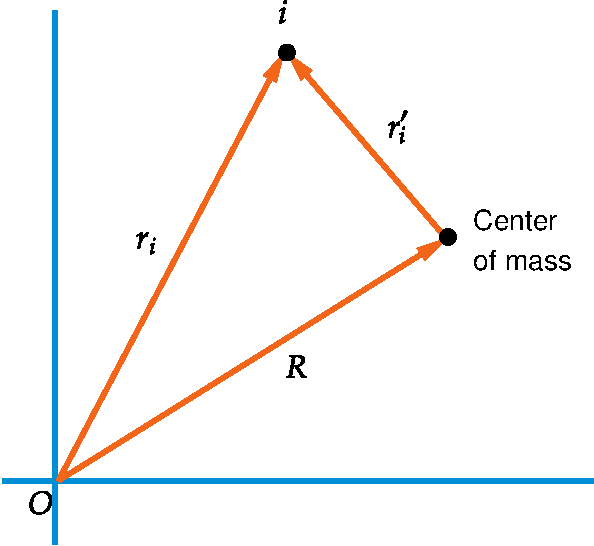
\includegraphics[height=4.5cm,width=5.5cm]{EP-02}
\end{figure}
\begin{align*}
\text{Let $R$ be the radius }&\text{vector from $O$ to the centre of mass to the $i^{th}$ particle}\\
\vec{r_1}&=\vec{r^\prime_1}+\vec{R}\\
\text{and}\quad
\vec{v_1}&=\vec{v^\prime_1}+\vec{\mathrm{v}}\\
\text{where}\quad
\mathrm{v}&=\frac{dR}{dt}\text{velocity of CM relative to $O$ }\\
\text{and}\quad
v^\prime_1&=\frac{dr^\prime}{dt}\\
\text{is the velocity of the $i^{th}$ }&\text{particle relative to centre of mass of the system}\\
\therefore \quad\text{total angular momentum}\\
\vec{L}&=\vec{R}\times M\vec{\mathrm{v}}+\sum\limits_{i}r^\prime_i\times p^\prime_i
\intertext{Total angular momentum about a point $O$ is the angular momentum of motion concentrated at the centre of mass, plus the angular momentum of motion about the centre of mass.}
\end{align*}
\begin{note}
	$L$ depends on origin $O$ through the vector $\vec{R}$ 
	only if the centre of mass is at rest with respect to $O$ will the angular momentum be independent of point of reference.
\end{note}
\textbf{Energy Equation}
\begin{align*}
\text{Work done by all forces in }&\text{moving a system from an initial configuration $1$ to a final configuration $2$}\\
W_{12}&=\sum\limits_{i}\int\limits_{1}^{2}\vec{F}_i\cdot d\vec{s}_i=\sum\limits_{i}\int\limits_{1}^{2}F_i^{(e)}\cdot d s_i+\sum\limits_{i,j ,i+j}\ \int\limits_{1}^{2}
F_{ji}\cdot ds_i\\
\text{by equation of }&\text{motion}\\
\sum\limits_{i}\int\limits_{1}^{2}\vec{F}_i\cdot d\vec{s}_i&=\sum\limits_{i}\int\limits_{1}^{2}m_i \vec{\dot{v}_i}\cdot\vec{v}_i dt=\sum\limits_{i}\int\limits_{1}^{2}r(\frac{1}{2}m_iv_i^2)\\
\therefore W_{12}&=T_2-T_1\\
\text{	Where $T$, the }&\text{total kinetic energy of system}\\
T&=\frac{1}{2} \sum\limits_{i}m v_i^2\\
\text{Transformation to}&\text{ centre of mass coordinates}\\
T&=\frac{1}{2} Mv^2+\frac{1}{2}\sum m_i {v^\prime}_i^2
\intertext{ie. kinetic energy obtained if all mass were concentrated at the centre of mass $+$	kinetic energy of motion about the centre of mass. When external forces are derivable in terms of the gradient of a potential the first term can be written as}
 \sum\limits_{i}\int\limits_{1}^{2}\vec{F}_i^{(e)}\cdot d {s}_i&=-\sum\limits_{i}\int\limits_{1}^{2}\nabla _i v_i\cdot d \vec{s}=-\sum\limits_{i}-v_i \Bigr |_{1}^{2}\\
 \text{If the internal forces are  }&\text{also conservative.}\\
 v_{ij}&=v_{ij}(|r_i-r_j|)\\
 \text{When forces are all }&\text{conservative}\\
 \sum\limits_{i,j ,i+j}\ \int\limits_{1}^{2}
 F_{ji}\cdot ds_i&=-\sum\limits_{i}\int\limits_{1}^{2}(\nabla _i v_{i j}\cdot d s_i+\nabla_j v_{ij}\cdot ds_i)\\
 \vec{r}_{ij}&=(r_i-r_j), \nabla_{i j}\text{ gradient with respect to }r_{i j}\\
  \text{ Then}{ \nabla_i} v_{ij}&={\nabla_{i j}} v_{ij} =-\nabla_j v_{ij}\\
 ds_i-ds_i&=dr_i-dr_i=dr_{ij}\\
\text{$\therefore $\quad total work arising}&\text{ from internal force}\\
&=\frac{-1}{2}\sum\limits_{i,j ,i+j}\ \int\limits_{1}^{2}\nabla_{i j} \nabla_{i j}\cdot d\vec{r}_{ij}\\
&=\frac{-1}{2}\sum\limits_{i,j ,i+j} v_{ij}\Bigr |_{1}^{2}
\intertext{ $\therefore$ \quad The external and internal force are both derivable from potentials so it is possible to define a total potential energy $v$ of the system.}
v&=\sum\limits_{i}v_i+\frac{1}{2}\sum\limits_{i,j ,i+j}v_{ij}
 \end{align*}

 
\begin{itemize}
	\item For rigid body internal potential is constant
	\item  In rigid body internal forces do no work.
\end{itemize}
\section{Constraints}
We have,
$$ m_i\ddot{\mathbf{r}}_1=\textbf{F}_1^{(e)}+\sum\limits_{j}\textbf{F}_{ji}$$
All problems in mechanics be reduced to solving a set of differential equation. But this view is over simplified even from a purely physical's standpoint \\
eg:it is necessary to take constraints\\\\
While solving a problem along with this we have to take consideration of constraints that limits the motion of the system.\\
Constraints are classified in various ways.\\\\
\begin{itemize}
\item \textbf{Holonomic Constraints}:  If the conditions of constraint can be expressed as equations connecting the coordinates of the particles (and possibly the time) having the form,
	$$ f(\textbf{r}_1,\textbf{r}_2, \textbf{r}_3,.....t)=0$$
	Then constraints are holonomic. Holonomic Constraint equations are integrable.
	\begin{example}
	rigid body $(\textbf{r}_i-\textbf{r}_j)^2-c_{ij}^2=0$,
	a particle constrained to move along any curve or on a given surface equation.
	\end{example}

\item \textbf{Non Holonomic Constraints }:
Constraint which are not expressible as an equation are non holonomic constraint. Non-holonomic constraints include nonintegrable differential constraints, constraint conditions involve higher order derivatives, or may in the form of inequality.\\
\begin{example}
	Aparticle placed on the surface of a sphere, walls of a gas container.
\end{example}
\item \textbf{Rheonomous Constraints}:
Rheonomous constraints are which the constraint equation contain time as an explicit variable.\\
\item \textbf{Scleronomous}: 
Constraints which the constraint equations are not ecplicity dependent on time.\\
\end{itemize}
\textbf{Because of Constraints}:\\\\
1) The coordinates $r_i$ are no longer independent, since they are connected by the equation of constraint hence equation of motion are not independent.\\\\
2)The forces of constraint are unknown and must be obtained from solution.\\
In case of holonomic constraints the first difficulty is solved by introduction of generalized coordinates.\\\\
\section{Generalized Coordinates}
\begin{itemize}
	\item A system of N-particles, free from constraints has $3N$ independent coordinates or degree of freedom. 
	\item If there exist holonomic constraints expressed in $k$ equations in the form,  $f(r_1,r_2.....t)=0$, we use these equations to eliminate $k$ of the $3N$ coordinates.
	\item We left with $3N-k$ independent coordinates and system said to have $3N-k$ degrees of freedom.
	\item Elimination of dependend variable is done by introduction of new $3N-k$ , independent variables $q_1,q_2.....q_{3N-k}$ in terms of which the old coordinates are expressed by equation of form.
\begin{align*}
	\textbf{r}_1=\textbf{r}_1(q_1,q_2&.......q_{3N-k}, t)\\
	&....\\
	&....\\
	\textbf{r}_N=\textbf{r}_N(q_1,q_2&.......q_{3N-k}, t)
\end{align*}
	These contain constraints implicitly. Generalized coordinates are different from conventional orthogonal coordinates. All sorts of quantities  may be involved to serve as generalized coordinates.
	\begin{note}
		If the constraint is non-holonomic the equations expressing the constraint cannot be used to eliminate the dependent coordinates.\\\\
		\textbf{e.g. } : Object rolling on a rough surface without slipping.
	\end{note}
	
\end{itemize}
\section{D'Alembert's Principle and Lagrange's Equations}
\subsubsection{Virtual Displacement}
A change in the configuration of the system as the result of any arbitrary infinitesimal change of the coordinates $\delta \textbf{r}_i$ consistent with the forces and constraints imposed on the system at the given instant $t$. The change is called virtual to distinguish it from the actual displacement of the system occurring in a time interval `dt' , during which the forces and constraints may be changing.
\subsection{Principle of Virtual Work}
For a system in equilibrium, total force on each particle  $\textbf{F}_i=0$\\
Then virtual work of $\textbf{F}_i$ in displacement $\delta \textbf{F}_i$
\begin{equation}
\sum\limits_{i}\textbf{F}_i\cdot\delta \textbf{r}_i=0\label{EP-01}
\end{equation}
\begin{align*}
\text{Let, } \textbf{F}_i&=\textbf{F}_i^{(a)}+\textbf{f}_i\hspace{2cm}\textbf{F}_i^{(a)}- \text{applied force}\\
&\hspace{3.7cm}\textbf{f}_i - \text{force of constraint}\\
\therefore \text{Eq.(\ref{EP-01}) becomes, } \sum_{i} \mathbf{F}_{i}^{(a)} \cdot \delta \mathbf{r}_{i}+\sum_{i} \mathbf{f}_{i} \cdot \delta \mathbf{r}_{i}&=0 \\
\end{align*}
 We now restrict ourselves to systems for which the net virtual work of constraints is zero. We therefore have as the condition for equilibrium of a system that the virtual work of the applied forces vanishes.
\begin{equation}
\qquad\sum_{i} \mathbf{F}_{i}^{(a)} \cdot \delta \mathbf{r}_{i}=0\label{EP-02}
\end{equation}
This is often called \textit{principle of virtual work.}
\subsection{D'Alembert's Principle}
Equation (\ref{EP-02})  only deals with statics. We want a condition involving general motion of the system\\
The equation of motion 
\begin{align*}
\textbf{F}_i&=\dot{\textbf{P}_i}\\
\implies \textbf{F}_i-\dot{\textbf{P}_i}&=0
\end{align*}
\textit{The particle in the system will be in equilibrium under a force equal to actual force plus a "reversed effective force" , $-\dot{\textbf{P}_i}$.}\\
$\therefore$  equation (\ref{EP-01}) becomes



\begin{align}
\sum\limits_{i}(\textbf{F}_i-\dot{\textbf{P}_i})\cdot\delta \textbf{r}_i=0 \label{EP-05}
\sum\limits_{i}(\textbf{F}_i^{(a)}-\dot{\textbf{P}_i})\cdot\delta \textbf{r}_i+\sum\limits_{i}\textbf{f}_i\cdot\delta \textbf{r}_i&=0
\intertext{For systems for which virtual work of the forces of constraint vanishes,}
\sum\limits_{i}(\textbf{F}_i^{(a)}-\dot{\textbf{P}_i})\cdot\delta \textbf{r}_i&=0 \label{EP-06}
\end{align}

Which is called \textit{D'Alembert's principle}\\\\
\textbf{Generalized Force}
\begin{align}
\text{The translation from }&\text{$r_i$ to $q_j$ language starts from the transformation equations}\notag\\
\textbf{r}_i&=\textbf{r}_i(q_1,q_2,...q_n,t)\label{EP-07}\\
\text{velocity $\textbf{v}_i$ in terms }&\text{of $\dot{q}_k$}\notag\\
\mathbf{v}_{i} &\equiv \frac{d \mathbf{r}_{i}}{d t}=\sum_{k} \frac{\partial \mathbf{r}_{i}}{\partial q_{k}} \dot{q}_{k}+\frac{\partial \mathbf{r}_{i}}{\partial t}\label{EP-08}\\
\text{similarly, the arbitrary virtual}&\text{ displacement $\delta r_i$ can be connected with the virtual displacement $\delta q_1$ by}\notag\\
\delta \mathbf{r}_{i}&=\sum_{j} \frac{\partial \mathbf{r}_{i}}{\partial q_{j}} \delta q_{j}\\
\text{In terms of generalized }&\text{coordinates the virtual work of $\textbf{F}_i$ becomes}\notag\\
\sum_{i} \mathbf{F}_{i} \cdot \delta \mathbf{r}_{i}&=\sum_{i, j} \mathbf{F}_{i} \cdot \frac{\partial \mathbf{r}_{i}}{\partial q_{j}} \delta q_{j}=\sum_{j} Q_{j} \delta q_{j}\label{EP-10}\\
\text{Where $Q_j$ are called the } &\text{component of the }\textit{generalized force}\notag \\
Q_{j}&=\sum_{i} \mathbf{F}_{i} \cdot \frac{\partial \mathbf{r}_{i}}{\partial q_{j}}\label{EP-11}
\end{align}
\textit{Just as $q$'s need not have the dimensions of length, so the $Q$'s do not necessarily have the dimensions of force, but $Q_j\delta q_j$ must always have the dimensions of work.}
\begin{note}
	No variation of time, $\delta t$ is involved here since a virtual displacement by definition considers only displacements of the coordinates.
\end{note}
\subsection{D'Alembert's Principle in Generalized Coordinates}
\begin{align}
\sum\limits_{i}(r_i^{(a)}-\dot{P}_i)\cdot\delta r_i&=0\text{ \quad is the D'Alembert's Principle.}\notag\\
\sum_{i} \dot{\mathbf{p}}_{i} \cdot \delta \mathbf{r}_{i}&=\sum_{i} m_{i} \ddot{\mathbf{r}}_{i} \cdot \delta \mathbf{r}_{i}\notag\\
&=\sum_{i, j} m_{i} \ddot{\mathbf{r}}_{i} \cdot \frac{\partial \mathbf{r}_{i}}{\partial q_{j}} \delta q_{j}\notag\\
\text{Now consider the}&\text{ relation,}\notag\\
\sum_{i} m_{i} \ddot{\mathbf{r}}_{i} \cdot \frac{\partial \mathbf{r}_{i}}{\partial q_{j}}&=\sum_{i}\left[\frac{d}{d t}\left(m_{i} \dot{\mathbf{r}}_{i} \cdot \frac{\partial \mathbf{r}_{i}}{\partial q_{j}}\right)-m_{i} \dot{\mathbf{r}}_{i} \cdot \frac{d}{d t}\left(\frac{\partial \mathbf{r}_{i}}{\partial q_{j}}\right)\right]\label{EP-12}\\
\text{interchanging differ}&\text{entiation with respect to $t$ and $q_j$,}\notag\\
 \frac{d}{d t}\left(\frac{\partial \mathbf{r}_{i}}{\partial q_{j}}\right) &=\frac{\partial \dot{\mathbf{r}}_{i}}{\partial q_{j}}=\sum_{k} \frac{\partial^{2} \mathbf{r}_{i}}{\partial q_{j} \partial q_{k}} \dot{q}_{k}+\frac{\partial^{2} \mathbf{r}_{i}}{\partial q_{j} \partial t}, \notag\\
&=\frac{\partial \mathbf{v}_{i}}{\partial q_{j}}
\text{ we have from equation }(\ref{EP-08})\notag\\
\frac{\partial \mathbf{v}_{i}}{\partial \dot{q}_{j}}&=\frac{\partial \mathbf{r}_{i}}{\partial q_{j}}\label{EP-13}\\
\text{substitution of these in}&\text{ equation (\ref{EP-12})}\notag\\
\sum_{i} m_{i} \ddot{\mathbf{r}}_{i} \cdot \frac{\partial \mathbf{r}_{i}}{\partial q_{j}}&=\sum_{i}\left[\frac{d}{d t}\left(m_{i} \mathbf{v}_{i} \cdot \frac{\partial \mathbf{v}_{i}}{\partial \dot{q}_{j}}\right)-m_{i} \mathbf{v}_{i} \cdot \frac{\partial \mathbf{v}_{i}}{\partial q_{j}}\right]\notag\\
\text{second term on the LHS of }&\text{equation (\ref{EP-06}) can be explanded into,}\notag\\
\sum_{j}\left\{\frac{d}{d t}\left[\frac{\partial}{\partial \dot{q} j}\left(\sum_{i} \frac{1}{2} m_{i} v_{i}^{2}\right)\right]\right. &\left. -\frac{\partial}{\partial q_{j}}\left(\sum_{i} \frac{1}{2} m_{i} v_{i}^{2}\right)-Q_{j}\right\} \delta q_{j}\notag\\
\sum_{i} \frac{1}{2} m_{i} v_{i}^{2}&=T\quad \text{ie. system kinetic energy}\notag\\
\text{$\therefore$ D'Alembert's principle}&\text{ becomes ,}\notag\\
\sum_{j}\left\{\left[\frac{d}{d t}\left(\frac{\partial T}{\partial \dot{q}_{j}}\right)-\frac{\partial T}{\partial q_{j}}\right]\right.& \left. -Q_{j}\right\} \delta q_{j}=0\label{EP-14}
\end{align}
\subsection{Lagrange's Equation}
Any virtual displacement $\delta q_j$ is independent of $\delta q_k.$\\
$\therefore$ \quad only way to hold equation \ref{EP-14} is for the individual coefficients to vanish.
\begin{align}
\frac{d}{d t}\left(\frac{\partial T}{\partial \dot{q}_{j}}\right)-\frac{\partial T}{\partial q_{j}}=Q_{j}\label{EP-15}\\
\text{There are $n$ such equations in all,}&\text{ When forces are derivable from scalar potential $V$}\notag\\
\mathbf{F}_{i}&=-\nabla_{i} V\notag\\
\text{Then the generalized forces can}&\text{ be written as}\notag\\
Q_{j}&=\sum_{i} \mathbf{F}_{i} \cdot \frac{\partial \mathbf{r}_{i}}{\partial q_{j}}=-\sum_{i} \nabla_{i} V \cdot \frac{\partial \mathbf{r}_{i}}{\partial q_{j}}\notag\\
\text{Which is partial derivative of }&\text{$-V(r_1,r_2...r_3,t)$ with respect to $q_j$}\notag\\
Q_{j}&=-\frac{\partial V}{\partial q_{j}} .\label{EP-16}\\
\text{$\therefore$ \quad equation \ref{EP-15} can be }&\text{rewritten as}\notag\\
\frac{d}{d t}\left(\frac{\partial T}{\partial \dot{q}_{j}}\right)-\frac{\partial (T-V)}{\partial q_{j}}&=0\\
\text{Potential $V$ does not depend on the}&\text{ generalized velocities }\notag\\
\therefore \text{we can write }\notag\\
\frac{d}{d t}\left( \frac{\partial (T-V)}{\partial \dot{q}_{j}} \right)  -\frac{\partial (T-V)}{\partial q_{j}}&=0\notag\\
\text{defining the Lagrangian $L$,as }L&=T-V\notag\\
\therefore \text{ equation \ref{EP-15} becomes }&\notag\\
\frac{d}{d t}\left(\frac{\partial L}{\partial \dot{q}_{j}}\right)-\frac{\partial L}{\partial q_{j}}&=0\notag\\
\text{expression refered to as }&\textit{"Lagrange's equations"}\notag
\end{align}
\begin{note}
	If $L(q,\dot{q},t)$ is an approximate Lagrangian and $F(q,t)$ is any differentiable function of the generalized coordinates and time, then
	$$L^{\prime}(q, \dot{q}, t)=L(q, \dot{q}, t)+\frac{d F}{d t}$$
	is a Lagrangian also resulting in the same equation of motion.
\end{note}
\section{Formulation of Lagrangian}
Lagrangian in different coordinate system:
Lagrangian of a system is defined as $L=T\left(q_{i}, \dot{q}_{i}, t\right)-V\left(q_{i}, \dot{q}_{i}, t\right)$, where $T$ and $V$ are functions of generalized coordinates, generalized velocities and time $t$.\\
\textbf{How to write a Lagrangian}\\\\
\textbf{Step 1:}\\
(a) Draw a Cartesian coordinate system with a suitable origin.
(b) Then disturb the system arbitrarily and fix the coordinates of individual particle with respect to origin.
(c) Write down kinetic energy and potential energy as discussed below.
If a system constitutes $p$ number of particle and position vector of the $p^{\text {th }}$ particle is given by $\vec{r}_{p}=x_{p} \hat{i}+y_{p} \hat{j}+z_{p} \hat{k}$, then kinetic energy of the system is given by
\begin{align*}
T&=\frac{1}{2} \sum_{P} m_{p}\left[\left(\dot{x}_{p}\right)^{2}+\left(\dot{y}_{p}\right)^{2}+\left(\dot{z}_{p}\right)^{2}\right] \text { and }\\
\text{potential }&\text{energy is given by}\\
V&=\sum_{p} V_{p}\left(x_{p}, y_{p}, z_{p}, \dot{x}_{p}, \dot{y}_{p}, \dot{z}_{p}\right)\\
\text{Lagrangian of the  }&\text{system is given by }L=T-V
\end{align*}
\textbf{Step 2:}\\
(a) Find the degree of freedom with the formula $\mathrm{DOF}=3 N-k$ as discussed in previous chapter.\\
(b) Number of degree of freedom is equivalent to minimum number of independent motion.\\
(c) Identify the independent motion with the help of symmetry of problem.\\
(d) Transform the Lagrangian of the system in suitable symmetry.\\
\begin{exercise}
If kinetic energy and potential energy is given by $T=\frac{1}{2} m\left(\dot{x}^{2}+\dot{y}^{2}\right)$ and $V=-m g y$ respectively.
	 \begin{tasks}(1)
		\task[\textbf{a.}] Write down Lagrangian of the system.
		\task[\textbf{b.}] Identify generalized coordinate and generalized velocity.
		\task[\textbf{c.}] Identify cyclic coordinate and discuss conservation of momentum.
		\task[\textbf{d.}]  Discuss equation of motion.
	\end{tasks}
\end{exercise}
\begin{answer}
\begin{align*}
\text{(a)} \quad L=T-V &\Rightarrow \frac{1}{2} m\left(\dot{x}^{2}+\dot{y}^{2}\right)-(-m g y) \Rightarrow \frac{1}{2} m\left(\dot{x}^{2}+\dot{y}^{2}\right)+m g y\\
\text{(b)} \text{ Generalized coordinate }q_{1}&=x, q_{2}=y\text{ generalized velocity} \dot{q}_{1}=\dot{x}, \dot{q}_{2}=\dot{y}\\
\text{(c)} \left(\frac{\partial L}{\partial q_{1}}\right)&=\left(\frac{\partial L}{\partial x}\right)=0, \text{so it is a cyclic coordinate}\\ 
\text{Then} \left(\frac{\partial L}{\partial \dot{x}}\right)&=p_{x}=m \dot{x},\\ \text{Identified as linear momentum in }&\text{$x$ direction is constant of motion.}\\
\left(\frac{\partial L}{\partial y}\right)&=m g \neq 0,\text{ so it is not cyclic coordinate}\\
\text{(d)} \frac{d}{d t}\left(\frac{\partial L}{\partial \dot{x}}\right)-\left(\frac{\partial L}{\partial x}\right)&=0 \\
\frac{d}{d t} m \dot{x}-0&=0 \Rightarrow m \dot{x}=c,\\
 \text{which is exactly explained} &\text{ in section (b)}\\
\frac{d}{d t}\left(\frac{\partial L}{\partial \dot{y}}\right)-\left(\frac{\partial L}{\partial y}\right)&=0 \\
 \frac{d}{d t} m \dot{y}-m g&=0 \Rightarrow m \ddot{y}-m g=0
\end{align*}
\end{answer}
\begin{exercise}
	1. Apply Lagrange's equation to find the equation of motion of a particle in space using \\
	(a). Cartesian coordinates. \\
	(b). plane polar coordinates.
\end{exercise}
\begin{answer}
	\begin{align*}
	\text{ (a).\quad The generalized }&\text{forces needed are $F_{x}, F_{y}$, and $F_{z}$. Then}\\
	T &=\frac{1}{2} m\left(\dot{x}^{2}+\dot{y}^{2}+\dot{z}^{2}\right), \\ \frac{\partial T}{\partial x} &=\frac{\partial T}{\partial y}=\frac{\partial T}{\partial z}=0, \\
	 \frac{\partial T}{\partial \dot{x}}&=m \dot{x},  \frac{\partial T}{\partial \dot{y}}=m \dot{y}, \quad \frac{\partial T}{\partial \dot{z}}=m \dot{z}, \\
	\text{ \quad and the equations }&\text{of motion are}\\
	\frac{d}{d t}(m \dot{x})&=F_{x}, \quad \frac{d}{d t}(m \dot{y})=F_{y}, \quad \frac{d}{d t}(m \dot{z})=F_{z}\\
	\text{(b).\quad Here we must express}&\text{ $T$ in terms of $\dot{r}$ and $\dot{\theta}$. The transformation equations are}\\
	x&=r \cos \theta\\
	y&=r \sin \theta\\
	\text{the velocities }&\text{are given by}\\
	\dot{x}&=\dot{r} \cos \theta-r \dot{\theta} \sin \theta,\\
	\dot{y}&=\dot{r} \sin \theta+r \dot{\theta} \cos \theta\\
	\text{The kinetic energy }T&=\frac{1}{2} m\left(\dot{x}^{2}+\dot{y}^{2}\right)\text{ then reduces formally to}\\
	T&=\frac{1}{2} m\left[\dot{r}^{2}+(r \dot{\theta})^{2}\right]
	\intertext{ the plane polar components of the velocity are $\dot{r}$ along $\mathbf{r}$, and $r \dot{\theta}$ along the direction perpendicular to $r$, denoted by the unit vector $\hat{\theta}$. Hence, the square of the velocity expressed in polar coordinates is simply $\dot{r}^{2}+(r \dot{\theta})^{2}$.}\\
	\text{the components of }&\text{the gencralized force are}\\
	Q_{r}&=\mathbf{F} \cdot \frac{\partial \mathbf{r}}{\partial r}=\mathbf{F} \cdot \hat{\mathbf{r}}=F_{r}\\
	Q_{\theta}&=\mathbf{F} \cdot \frac{\partial \mathbf{r}}{\partial \theta}=\mathbf{F} \cdot r \hat{\mathbf{\theta}}=r {F}_{\theta} .
	\intertext{ There are two generalized coordinates, and therefore two Lagrange equations. The derivatives occurring in the $r$ equation are}
	\frac{\partial T}{\partial r}&=m r \dot{\theta}^{2}, \quad \frac{\partial T}{\partial \dot{r}}=m \dot{r}, \quad \frac{d}{d t}\left(\frac{\partial T}{\partial \dot{r}}\right)=m \ddot{r},\\
	m \ddot{r}-m r \dot{\theta}^{2}&=F_{r},\\
	\frac{\partial T}{\partial \theta}&=0, \quad \frac{\partial T}{\partial \dot{\theta}}=m r^{2} \dot{\theta}, \quad \frac{d}{d t}\left(m r^{2} \dot{\theta}\right)=m r^{2} \ddot{\theta}+2 m r \dot{r} \dot{\theta}.\\
	\frac{d}{d t}\left(m r^{2} \dot{\theta}\right)&=m r^{2} \ddot{\theta}+2 m r \dot{\theta} \dot{\theta}=r F_{\theta} .\\
	\text{where angular momentum }L&=m r^{2} \theta\text{ and torque }N^{(e)}=r F_{\theta}.
	\end{align*}
\end{answer}
\begin{exercise}
	Atwood's machine \\
	\begin{figure}[H]
		\centering
		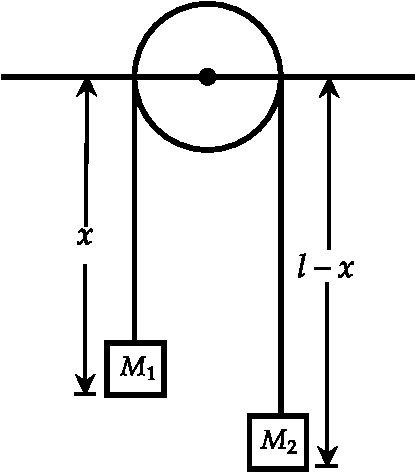
\includegraphics[height=4.7cm,width=4cm]{EP-04}
	\end{figure}
\end{exercise}
\begin{answer}
	\begin{align*}
	\intertext{A conservative system with holonomic, scleronomous constraint  (the pulley is assumed frictionless and massless). There is only one independent coordinate $x$, the position of the other weight being determined by the constraint that the length of the rope between them is $l$. The potential energy is}
	V&=-M_{1} g x-M_{2} g(l-x)\\
	\text{while the kinetic}&\text{ energy is}\\
	T&=\frac{1}{2}\left(M_{1}+M_{2}\right) \dot{x}^{2}\\
	\text{Lagrangian has}&\text{ the form}\\
	L&=T-V=\frac{1}{2}\left(M_{1}+M_{2}\right) \dot{x}^{2}+M_{1} g x+M_{2} g(l-x)\\
	\text{equation of}&\text{ motion}\\
	\frac{\partial L}{\partial  x}&=\left(M_{1}-M_{2}\right) g\\
	\frac{\partial  L}{\partial  x}&=\left(M_{1}+M_{2}\right) \dot{x}\\
	\text{$\mathrm{so}$\quad}\\
	\left(M_{1}+M_{2}\right) \ddot{x}&=\left(M_{1}-M_{2}\right) g,\\
	\ddot{x}&=\frac{M_{1}-M_{2}}{M_{1}+M_{2}} g,\\
	\end{align*}
\end{answer}
\begin{exercise}
	A bead (or ring ) sliding on a uniformly rotating wire in a force-free space. The wire is straight, and is rotated uniformly about some fixed axis perpendicular to the wire.
\end{exercise}
\begin{answer}
	\begin{align*}
	\intertext{This is an example of constraint being time dependent, with the rotationaxis along $z$ and the wire in the $xy$ plane.} 
	x&=r \cos \omega t \hspace{3cm}(\omega=\text { angular velocity of rotation }) \\
	y&=r \sin \omega t \hspace{3cm}(r=\text{distance along wire from rotation axis} )\\
	\text{constraint can be }&\text{expressed as $\dot{\theta}=\omega$, so}\\
	T&=\frac{1}{2} m\left(\dot{r}^{2}+r^{2} \omega^{2}\right)\\
	\text{The equation of motion}&\text{ is then}\\
	m \ddot{r}&-m r^{2}=0\\
	\ddot{r}&=r \omega^{2}  
	\intertext{which is the familiar simple harmonic oscillator equation with a change of sign. The solution $r=e^{\omega t}$ for a bead initially at rest on the wire shows that the bead moves exponentially outwards.The angular momentum, $L=m r^{2} \omega=m \omega r_{0}^{2} e^{2 \omega t}$, provides the force $F=N / r$, which produces the constraint force, $F=2 m r_{0} \omega^{2} e^{\omega t}$, acting perpendicular to the wire and the axis of rotation.}
	\end{align*}
\end{answer}